\documentclass[tikz,12pt]{beamer}

\mode<presentation>
{
  \usetheme{Frankfurt}
}

\usepackage[utf8]{inputenc}
%\usepackage[orientation=portrait,size=custom,width=91.4,height=121.9]{beamerposter}
\usepackage[orientation=portrait,size=a0,scale=1.4]{beamerposter}
\usepackage{lmodern}
\usepackage{listings}
\usepackage{color}
\usepackage{tikz}
\usepackage{amsmath}
\usepackage{hyperref}
\usepackage{color}

\usecolortheme{crane}
\setbeamertemplate{blocks}[rounded][shadow=false]
\hypersetup{
  colorlinks = true,
  linkcolor = blue,
  urlcolor = blue
}
\tikzstyle{every picture}+=[remember picture]
\usepackage{mdframed}
\usepackage{graphicx}
\graphicspath{{figures/}}
\usetikzlibrary{arrows,shapes}
\usefonttheme{professionalfonts}

\definecolor{dkgreen}{rgb}{0,0.6,0}
\definecolor{gray}{rgb}{0.5,0.5,0.5}
\definecolor{mauve}{rgb}{0.58,0,0.82}
\definecolor{yaleblue}{rgb}{0.06, 0.3, 0.57}

\definecolor{belgium2}{HTML}{3D3D3D}
\definecolor{france2}{HTML}{2A7BB4}
\definecolor{germany2}{HTML}{146F19}
\definecolor{netherlands2}{HTML}{D6EA33}

\lstset{
  language=R,
  aboveskip=3mm,
  belowskip=3mm,
  showstringspaces=false,
  columns=flexible,
  basicstyle={\small\ttfamily},
  numbers=none,
  numberstyle=\tiny\color{gray},
  keywordstyle=\color{blue},
  commentstyle=\color{dkgreen},
  stringstyle=\color{mauve},
  breaklines=true,
  breakatwhitespace=true,
  tabsize=3
}
\setbeamercolor{block title}{bg=yaleblue, fg=white}
\setbeamerfont{block title}{size=\large,series=\bf}

\setbeamertemplate{block begin}{
%  \vskip.75ex
  \begin{beamercolorbox}[leftskip=1cm,colsep*=.75ex]{block title}%
    \usebeamerfont*{block title}\insertblocktitle
  \end{beamercolorbox}%
  {\ifbeamercolorempty[bg]{block body}{}{\nointerlineskip\vskip-0.5pt}}%
  \usebeamerfont{block body}%
  \begin{beamercolorbox}[colsep*=.75ex,sep=.75ex,vmode]{block body}%
    \ifbeamercolorempty[bg]{block body}{\vskip-.25ex}{\vskip-.75ex}\vbox{}%
  }
  \setbeamertemplate{block end}{
  \end{beamercolorbox}
}

\newenvironment<>{varblock}[2][.9\textwidth]{%
  \setlength{\textwidth}{#1}
  \begin{actionenv}#3%
    \def\insertblocktitle{#2}%
    \par%
    \usebeamertemplate{block begin}}
  {\par%
    \usebeamertemplate{block end}%
  \end{actionenv}}

\title{\Huge Short-term forecasting with dynamic factor models}
\author{\large Rytis Bagd\v{z}i\={u}nas, Aspirant FNRS}
\institute{\normalsize CORE, Universit\'{e} catholique de Louvain, Belgium}
\date{}
\usepackage{geometry}

\addtolength{\oddsidemargin}{1cm}
\addtolength{\evensidemargin}{1cm}
\addtolength{\topmargin}{-1.8cm}
\begin{document}
\begin{frame}[fragile, t]{} 

  \tikzstyle{na} = [baseline=.5ex]

  \maketitle


\begin{columns}[t]
  \begin{column}{.41 \linewidth}
    \begin{block}{\large Initial problem}
      Predict economic growth (\textbf{GDP}), \textbf{inflation} and other summary variables in the short-term. Construct an index representing current state of the economy. Some challenges to take into account:
      \begin{itemize}
      \setlength{\itemindent}{1.2em}
      \setlength{\parskip}{4pt}
      \item integrate large number of time series
      \item asynchronous data arrival
      \item deal with NAs
      \item mixed-frequency nature of data
      \item possible regime changes, e.g. boom and bust cycles
      \item identification and economic constraints
    \end{itemize}
    \end{block}
    \vspace{3cm}
    \begin{block}{\large Getting data with \texttt{rsdmx}}
    Statistical data and metadata exchange (\texttt{SDMX}) standard has been sponsored by ECB, Eurostat, IMF, OECD, etc.
  
    \vspace{0.5cm}
    \texttt{rsdmx} package aims to fully implement \texttt{SDMX-ML} standard in \texttt{R}:
    \vspace{0.5cm}
    \begin{itemize}
      \setlength{\itemindent}{1.2em}
      \setlength{\parskip}{6pt}
      \item \texttt{readSDMX} downloads and parses \texttt{XML} data and metadata
      \item \texttt{as.data.frame} converts \texttt{SDMXData} object to a data.frame
    \end{itemize}
    \vspace{0.5cm}
    \texttt{rsdmx} is still under development but already very useful. In the future, it seeks to implement \texttt{writeSDMX}, automate timestamp treatment and assist in query construction.
  \end{block}
  \underline{Example}: $767$ monthly business and consumer surveys for OECD and partner countries are downloaded in seconds.
  \begin{flushright}\tikz[baseline]{\node[fill=blue!20](a2) {Sample plot}}\end{flushright}
  \begin{lstlisting}
  library(rsdmx)
  url <- "http://stats.oecd.org/restsdmx/sdmx.ashx/GetData/"
  key <- "MEI_BTS_COS/..BLSA.M/all?startTime=2014-Q4"
  xml_data <- readSDMX(paste0(url,key))
  data <- as.data.frame(xml_data)
  \end{lstlisting}

  \rule{1.0 \linewidth}{0.4pt}
  \vspace{0.1cm}

  \begin{block}{\large Our objectives}
    \begin{itemize}
    \setlength{\itemindent}{0.5em}
    \item[$\Rightarrow$] Package for \texttt{R} that facilitates the estimation part: \textbf{dynfactoR}
    \end{itemize}

    \textit{Why}? Current ``libraries'' for dynamic factor model estimation are scattered and mostly Matlab-only. \underline{State-space modelling} is already available for \texttt{R} but exploiting dynamic factor model structure will lead to gains in efficiency.
    \end{block}

    \vspace{1cm}

    The following snippet estimates a dynamic factor model with a single regime where $2$-dimensional factor $\mathbf{X}_{t}$ is assumed to follow VAR(2). This model is statistically identified since $\mathbf{Q} = \operatorname{Id}$ and $\mathbf{F}$ is partially upper triangular. See Bai \& Wang (2012).
    \vspace{1cm}
    \begin{lstlisting}
    library(dynfactoR)
    DFMfit <- dfm(data, f=2, p=2, rF='upper', rQ='identity')
    summary(DFMfit, plot=TRUE)
    \end{lstlisting}
    \begin{flushright}\tikz[baseline]{\node[fill=blue!20](a1) {Result}}\end{flushright}
    \begin{itemize}
      \setlength{\itemindent}{0.5em}
      \item Restrictions on $\mathbf{F}$ can be specified to deal with mixed-frequency, identification and other constraints.
      \item Kalman filtering supports missing data and asynchronous updates
    \end{itemize}

    \vspace{1.5cm} 

  
    \begin{block}{References}
      \begin{enumerate}
      \setlength{\itemindent}{0.2em}
      \item Stock \& Watson (2002). \textit{Forecasting using principal components from a large number of predictors.}
      \item Doz, Gianone \& Reichlin (2006). \textit{A quasi-maximum likelihood approach for large approximate dynamic factor models.}
      \item Bai \& Wang (2012). \textit{Identification and estimation of dynamic factor models.}
      \item Banbura \& Modugno (2014). \textit{Maximum likelihood estimation of factor models on datasets with arbitrary pattern of missing data.}
      \end{enumerate}
    \end{block}
  \end{column}
  
  \begin{column}{.45 \linewidth}
    \begin{flushleft}
    \begin{figure}
      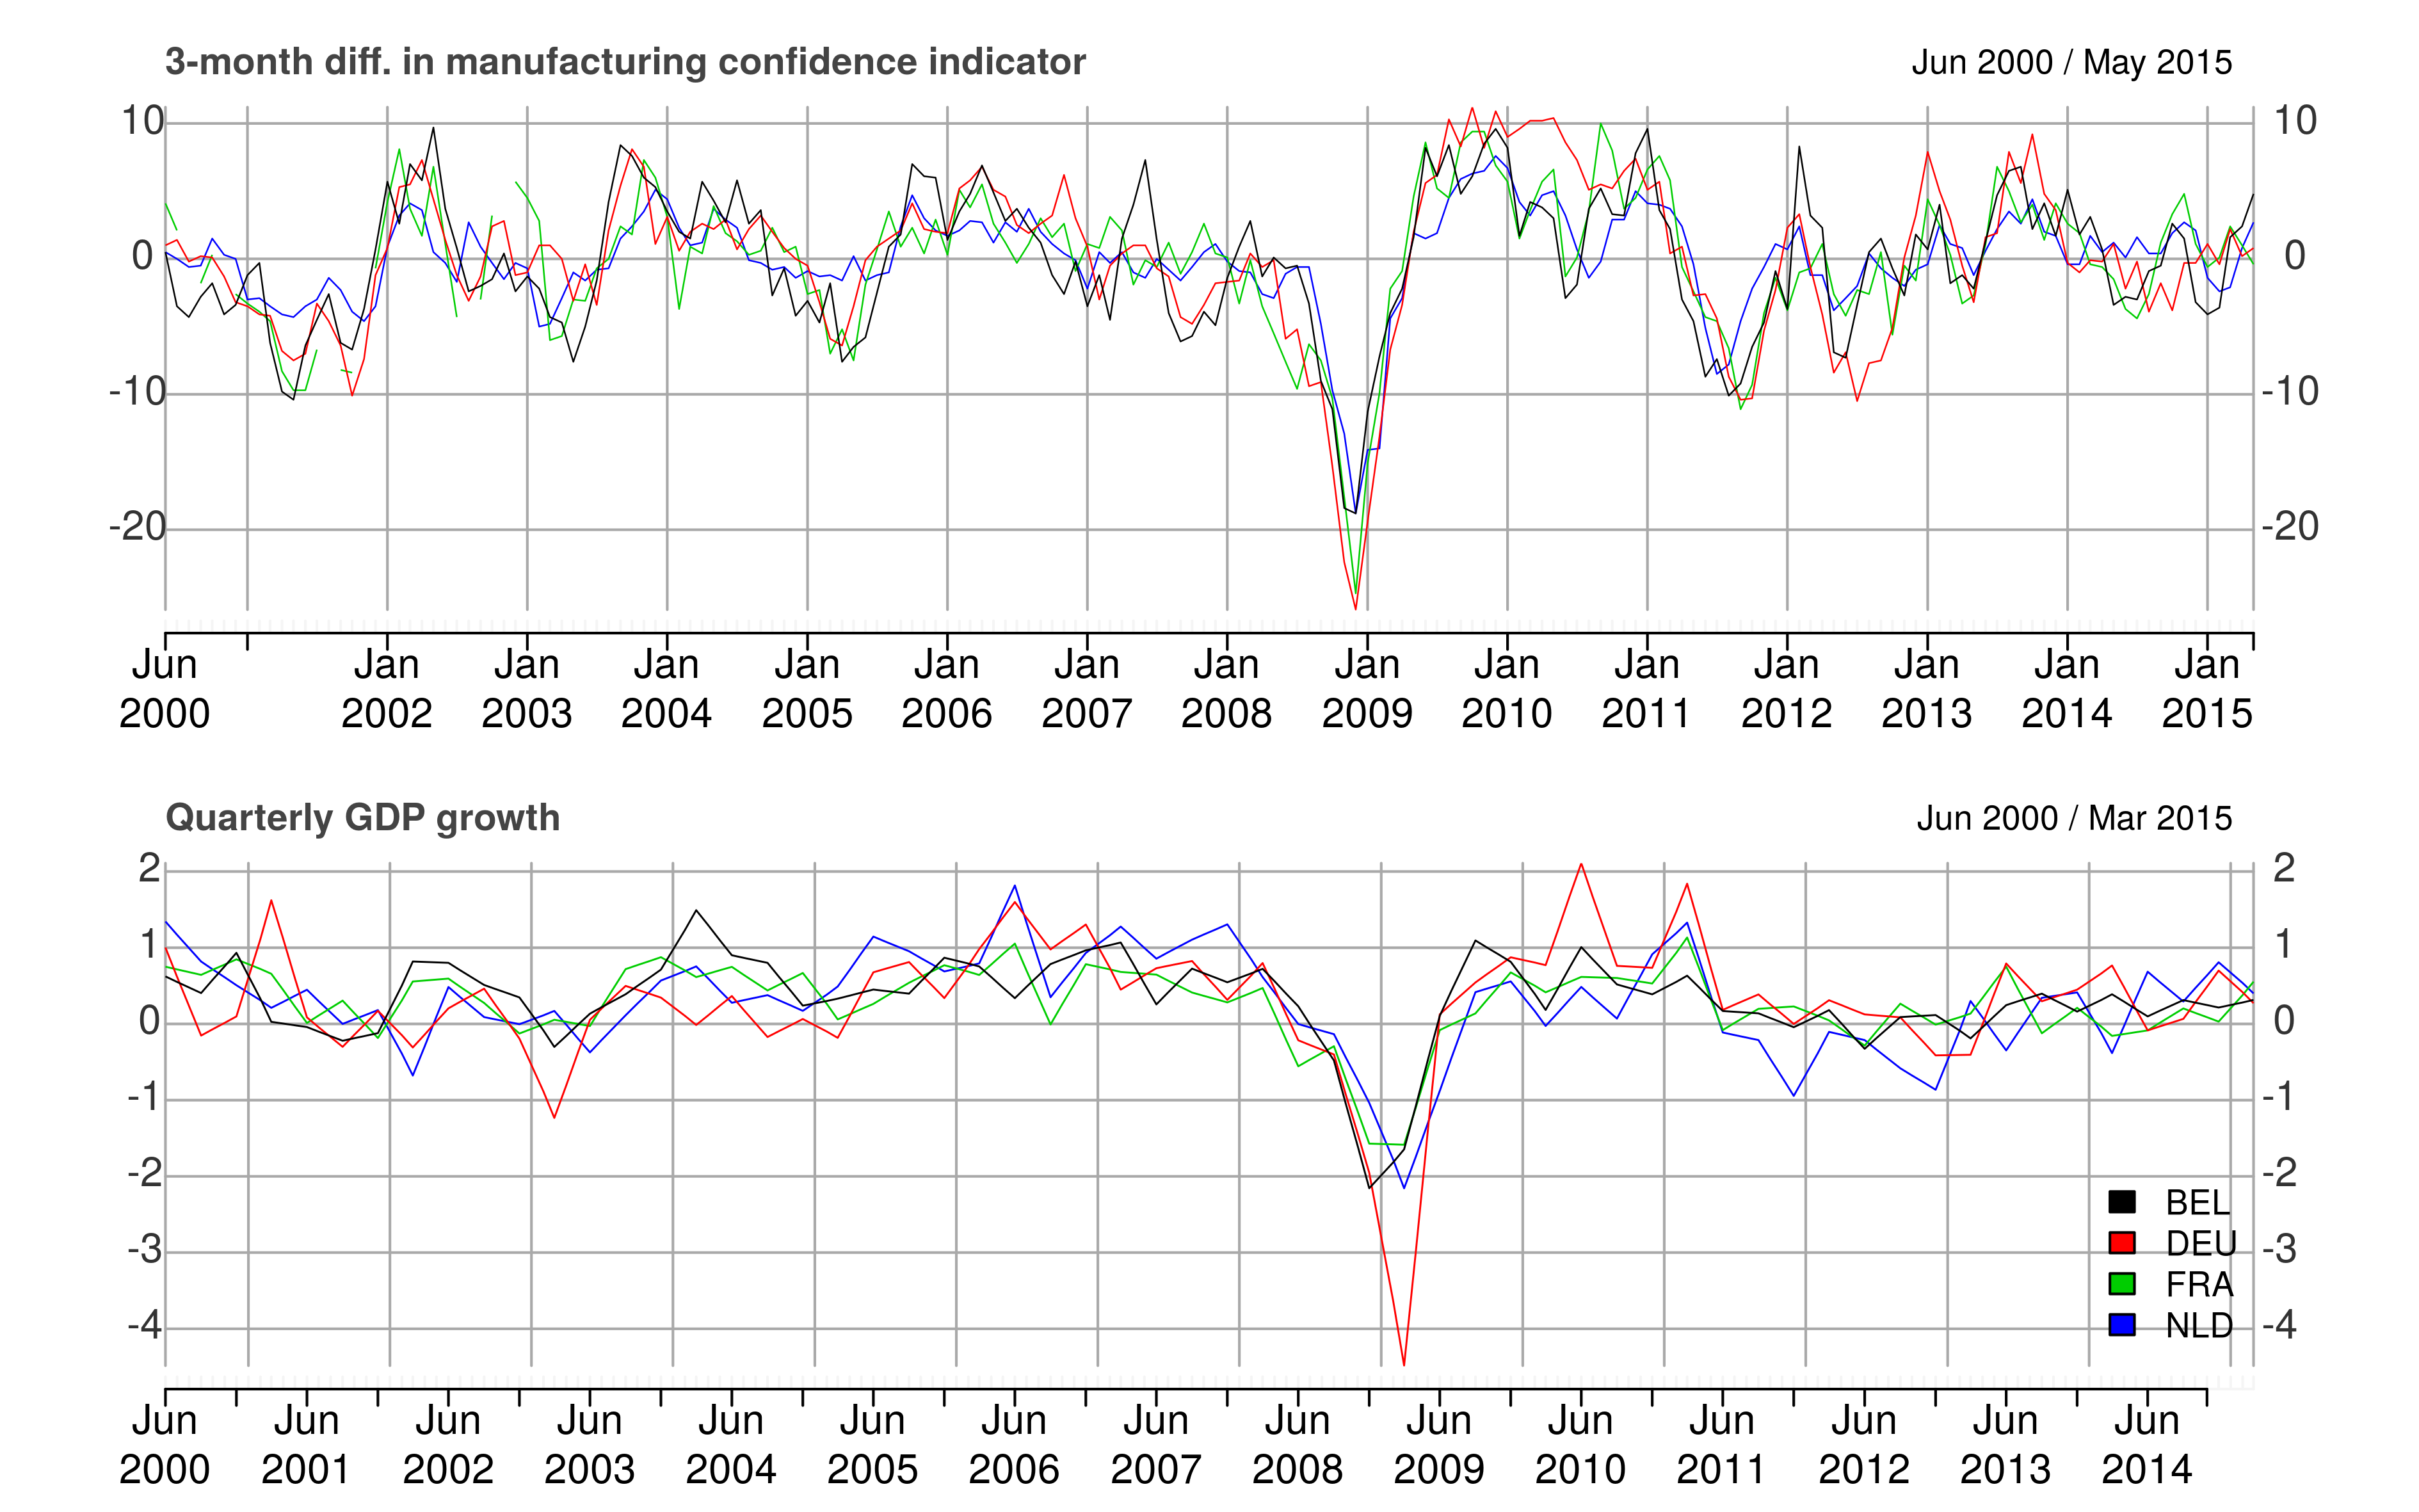
\includegraphics[scale=1.5]{comparison2}
      \caption{\textbf{Top}: monthly manufacturing survey data in Belgium, \textcolor{red}{Germany}, \textcolor{green}{France} and \textcolor{blue}{the Netherlands}. \textbf{Bottom}: quarterly GDP growth. It looks as if there was a common underlying pattern.}
    \end{figure}
    \end{flushleft}
    \tikz[na]{\node[fill=blue!20](t2) {\textit{Source}: OECD}}
    \begin{flushleft}\rule{1.0 \linewidth}{0.4pt}\end{flushleft}
  \vspace{0.5cm}
  \begin{varblock}[35cm]{\large Modelling solution: dynamic factor models}
    Let $\mathbf{Y}_{t}$ be a high-dimensional dataset and $\mathbf{X}_{t}$ an unobservable latent low-dimensional process such that
    \begin{align*}
      \mathbf{Y}_{t} &= \mathbf{F}_{s_{t}}\mathbf{X}_{t} + \boldsymbol\varepsilon_{t} \\ 
      \mathbf{X}_{t} &= \mathbf{A}_{1,s_{t}}\mathbf{X}_{t-1} + \dots + \mathbf{A}_{p,s_{t}}\mathbf{X}_{t-p} + \mathbf{u}_{t} 
    \end{align*}
    with $\boldsymbol\varepsilon_{t} \sim \mathcal{N}\left(0, \mathbf{R}\right)$ and $\mathbf{u}_{t} \sim \mathcal{N}\left(0, \mathbf{Q}\right)$. $\left(\mathbf{F}_{s_{t}}, \mathbf{A}_{1:p,s_{t}}\right)$ may also switch regime $s_{t} \in \left\lbrace 0, 1 \right\rbrace$ with $s_{t}$ following a Markov-switching process.
    \vspace{0.5cm}
  
    This model is \textbf{flexible} enough to deal with most issues stated initially.
  \end{varblock}
  \vspace{2cm}
    \begin{block}{\large Useful to know beforehand}
    \begin{itemize}
      \setlength{\parskip}{4pt}
      \item \textbf{Pre-processing} \\ Normalize and deseasonalize $\mathbf{Y}_{t}$, e.g. \texttt{x12} package in \texttt{R} can do batch processing with \texttt{X13-ARIMA-SEATS} methodology
      \item \textbf{Identification} \\ If statistical identification is an issue, impose constraints on $\left(\mathbf{F},\mathbf{R},\mathbf{Q}\right)$.
      \item \textbf{Estimation methods} \\ Based on Kalman filter and Kim filter (still experimental!) for Markov-switching case
         \begin{itemize}
            \item Maximizing likelihood with non-linear optimization procedures
            \item EM-algorithm
          \end{itemize}
    \end{itemize}
    \end{block}
    \vfill
    \tikz[na]{\node[fill=blue!20](t1) {First dynamic factor and trend for 2 months-ahead}}
   \begin{figure}
      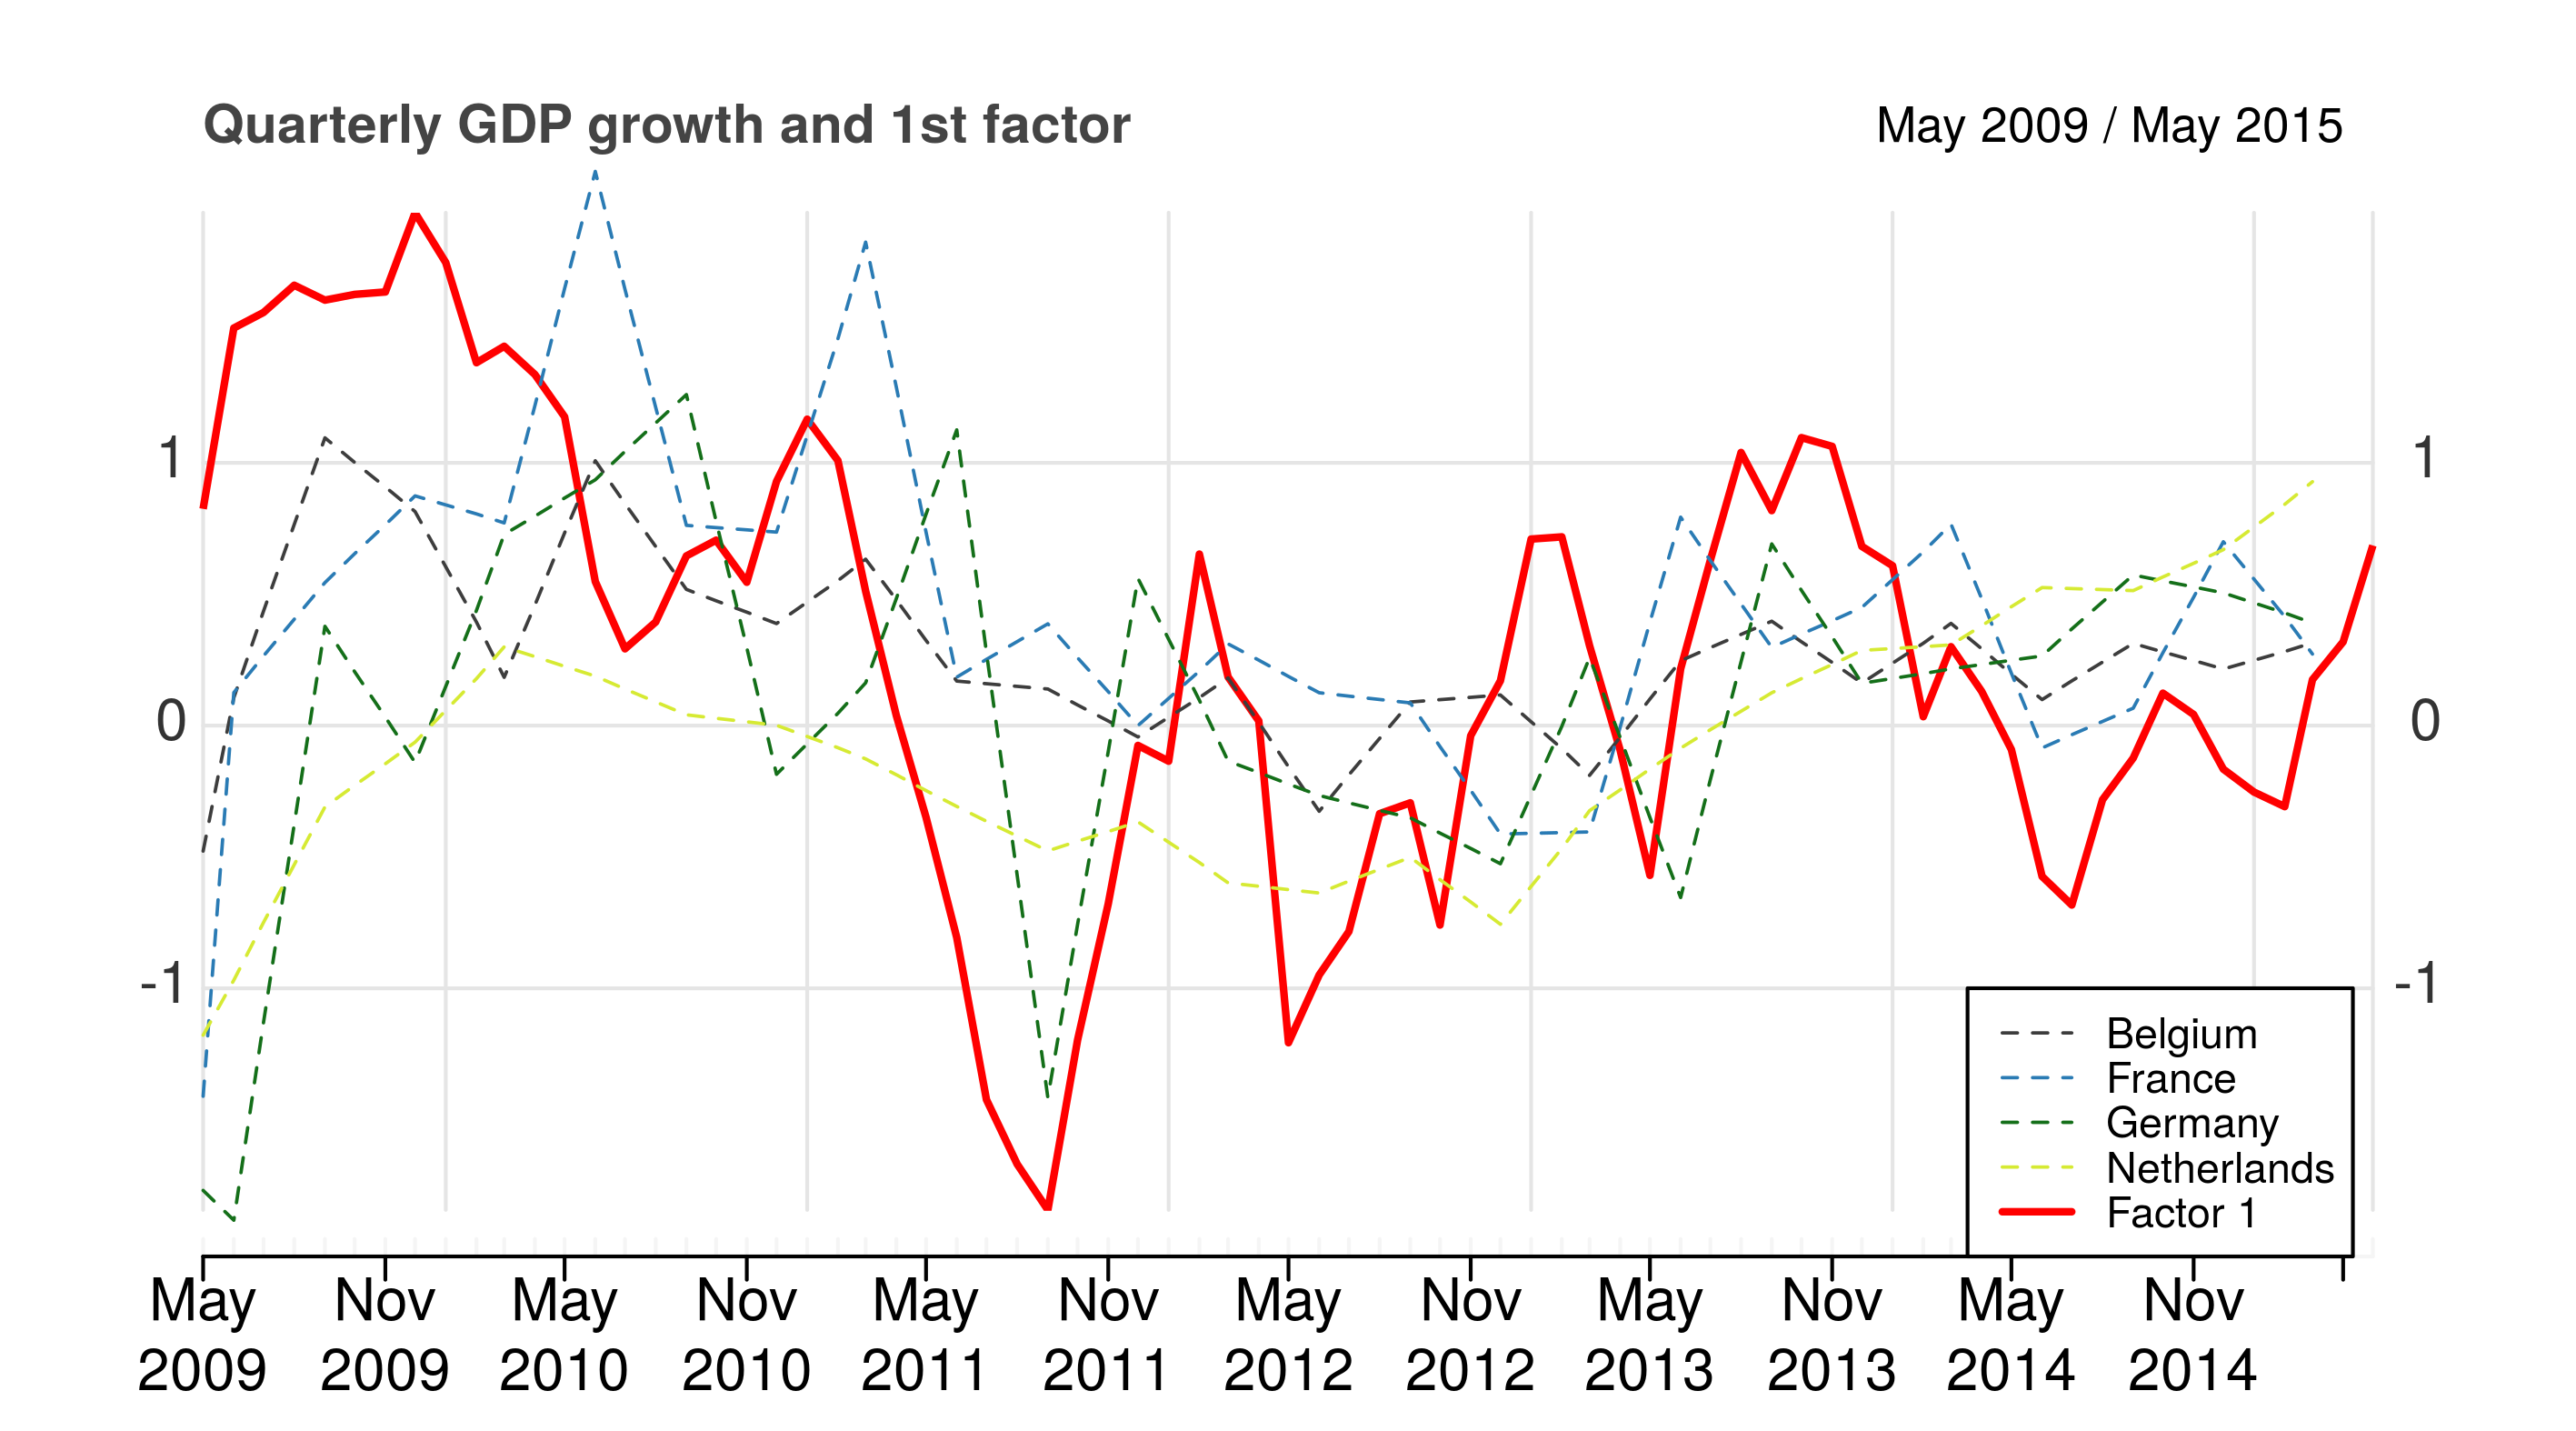
\includegraphics[scale=1.7]{factor2}
      \caption{Quarterly GDP growth in \textcolor{belgium2}{Belgium}, \textcolor{france2}{France}, \textcolor{germany2}{Germany} and \textcolor{netherlands2}{the Netherlands}. \textcolor{red}{First factor} often precedes trend variations in GDP data.}
    \end{figure}
   \begin{flushleft}\rule{1.0 \linewidth}{0.4pt}\end{flushleft}
   \begin{columns}[t]
      \begin{column}{.85 \linewidth}
    \begin{mdframed}
    \begin{itemize}
      \item Source for this poster and other projects: \href{http://github.com/rbagd}{rbagd@github}
      \item Tutorial on using SDMX from R: \href{http://rbagd.eu}{rbagd.eu}
      \item \texttt{rsdmx} is available on CRAN: its developer Emmanuel Blondel would appreciate any programming and financial assistance!
    \end{itemize}
  \end{mdframed}
  \end{column}
  \begin{column}{.13 \linewidth}
    \begin{figure}
      
\includegraphics[scale=0.15]{uclouvain.jpg}
      \hspace{1cm}
      
\includegraphics[scale=0.5]{fnrs.jpg}
    \end{figure}
  \end{column}
  \end{columns}
\end{column}
\end{columns}

\begin{tikzpicture}[overlay]
  \draw[->,gray!70] (a1) edge [bend left] (t1);
  \draw[->,gray!70] (a2) to [bend left=20] (t2);
\end{tikzpicture}


\end{frame}
\end{document}
